\documentclass{abnt-uefs} % Classe de formatação da UEFS
\usepackage[utf8]{inputenc}
%\usepackage[T1]{fontenc}
\usepackage[call=authordata,alf,abnt-emphasize=bf,abnt-etal-text=emph,abnt-and-type=&,abnt-etal-list=3,abnt-etal-cite=3,recuo=0.0cm]{abntcite}
\usepackage[brazil]{babel}
\usepackage{mathptmx}
\usepackage[pdftex]{graphicx}
%\usepackage[small,bf]{caption}
\usepackage{longtable}
\usepackage{array}
\usepackage{amssymb,amsmath,amsthm,amsfonts}
%\usepackage{textcomp}
%\usepackage{textcase} 
\usepackage{float} % para as figuras ficarem onde foram colocadas no latex - deve colcoar na figura [H]
\usepackage{color}
%\usepackage{url}
\usepackage{nameref}
\usepackage{color}   %May be necessary if you want to color links
\usepackage{amsmath}

%Gambiarra das imagens
\usepackage{placeins}
\usepackage{tikz}
\let\Oldsection\section
\renewcommand{\section}{\FloatBarrier\Oldsection}

\let\Oldsubsection\subsection
\renewcommand{\subsection}{\FloatBarrier\Oldsubsection}

\let\Oldsubsubsection\subsubsection
\renewcommand{\subsubsection}{\FloatBarrier\Oldsubsubsection}

%Tirar negrito do título das imagens


% Colocar links nos capítulos
%\usepackage{hyperref}
%\hypersetup{
%	colorlinks=true, %set true if you want colored links
%	linktoc=all,     %set to all if you want both sections and subsections linked
%	linkcolor=blue,  %choose some color if you want links to stand out
%}
%\makeatletter
%\newcommand*{\updatelabelname}[1]{% For correcting \@currentlabelname, if needed
%	\xdef\@currentlabelname{#1}}
%\makeatother


%%%%%%%%%%%%%%%%%%%%%%%%%%%%%%%%%%%
% Configuração de código fonte
% Colorido
\usepackage{color}
\usepackage{bold-extra}
\usepackage{listings}
\definecolor{dkgreen}{rgb}{0,0.6,0}
\definecolor{gray}{rgb}{0.5,0.5,0.5}
\definecolor{mauve}{rgb}{0.58,0,0.82}
\lstset{
	language=c++, % Replace
	basicstyle={\footnotesize\ttfamily},
	keywordstyle={\bfseries\color{blue}},
	commentstyle=\color{dkgreen},
	stringstyle={\slshape\color{mauve}},
	numberstyle=\footnotesize,
	numbers=left,
	showstringspaces=false,
	breaklines=true,
	tabsize=4,
	frame=tb
}

\renewcommand{\lstlistingname}{Algoritmo}% Listing -> Algorithm
\renewcommand{\lstlistlistingname}{Lista de \lstlistingname s}
\makeatletter
\renewcommand{\l@lstlisting}[2]{%
	%\@dottedtocline{1}{0em}{1.5em}{\lstlistingname\ #1}{#2}%
	\leftskip 3.1em
	\rightskip 1.6em
	\parfillskip -\rightskip
	\parindent 0em
	\@tempdima 2.0em
	\advance\leftskip \@tempdima \nobreak\hskip -\leftskip %%Tinha \null\nobreak\..
	{Algoritmo \normalfont #1}\nobreak \tabfillnum{#2}
	
}
\makeatother

\usepackage{csquotes}

			
% Preto e branco
%\usepackage{xcolor}
%\usepackage{bold-extra}
%
%\usepackage{listings}
%\lstset{
%	language=c, %Replace
%	basicstyle={\footnotesize\ttfamily},
%	keywordstyle=\bfseries,
%	commentstyle=\color{black!75},
%	stringstyle=\slshape,
%	numberstyle=\footnotesize,
%	numbers=left,
%	showstringspaces=false,
%	breaklines=true,
%	tabsize=4,
%	frame=tb
%}


\usepackage{enumitem}
\setlist{
	listparindent=\parindent,
	parsep=0pt,
}

\graphicspath{{./figuras/}} % Diretório padrão de figuras.
%%%%%%%%%%%%%%%%%%%%%%%%%%%%%%%%%%%%%%%%%%%%%%%%%%%%%%%%%%%%%%%%%%%%%%%%%%%%%%%
% Este arquivo faz parte do template de Relatório Parcial baseado nas normas da ABNT 
%  voltado para alunos da UEFS
% Desenvolvimento: Danilo de Oliveira Gonçalves
% Adaptação final: João Carlos Nunes Bittencourt
% Data: 31/03/2011
% Atualização: 30/11/2011
% Descrição do arquivo:
%   Esse arquivo apresenta as definições de constantes que formarão a capa e 
%   a folha de rosto. Siga as instruções e modifique de acordo com o que
%   lhe foi orientado.
%%%%%%%%%%%%%%%%%%%%%%%%%%%%%%%%%%%%%%%%%%%%%%%%%%%%%%%%%%%%%%%%%%%%%%%%%%%%%%%

% ---------- Preambulo ----------
\instituicao{Centro Universitário Serra dos Órgãos – UNIFESO} % nome da instituicao
\fundacao {Fundação Educacional Serra dos Órgãos – FESO} % Fundação
\departamento{CENTRO DE CIÊNCIAS E TECNOLOGIA – CCT}
\graduacao{Curso DE BACHARELADO EM CIÊNCIA DA COMPUTAÇÃO} % nome do curso
\curso{Ciência da Computação}

\documento{Trabalho de Conclusão de Curso} % tipo de documento
\titulacao{Bacharel} % [Bacharel]

\titulo{Técnicas de otimização de programação dinâmica} % titulo do trabalho em portugues
%\subtitulo{Sub-título, se necessário} % caso necessário um sub-título, utilize este campo
\title{Title in English} % titulo do trabalho em ingles

\autor{Gabriel Lagoa Duarte} % autor do trabalho
\cita{DUARTE, Gabriel} % sobrenome (maiusculas), nome do autor do trabalho

\palavraschave{Programação dinâmica. Otimização. Maratona de programação. \textit{Convex Hull Trick}} % palavras-chave do trabalho, separados por ponto
\keywords{Dynamic Programming. Optimization. Programming contest. Convex Hull Trick} % palavras-chave do trabalho em ingles, separados por ponto

\comentario{\UEFSdocumentodata\ apresentado ao \ABNTinstituicaodata\ como requisito obrigatório para obtenção do título de \UEFStitulacaodata\ em \UEFScursodata.}

\orientador{Rafael Gomes Monteiro} % nome do orientador do trabalho
%\orientador[Orientadora:]{Nome da Orientadora} % <- no caso de orientadora, usar esta sintaxe
\coorientador{} % nome do co-orientador do trabalho, caso exista
%\coorientador[Co-orientadora:]{Nome da Co-orientadora} % <- no caso de co-orientadora, usar esta sintaxe

\local{Teresópolis} % cidade
\data{2017} % ano

% Termo Aprovação

\textoaprovacao{\UEFSdocumentodata\ aprovado como requisito parcial para obtenção do título de \UEFStitulacaodata\ no \ABNTinstituicaodata\ pela banca examinadora:}

\primeiroassina{Rafael Gomes Monteiro (Orientador), M.Sc.}

\segundoassina{Eugênio da Silva, D.Sc.}

\terceiroassina{Hermano Lourenço Souza Lustosa, M.Sc.}

\localdia{Teresópolis}
\mesdia{22 de novembro de 2017}

% DECLARAÇÃO DE PRÓPRIA AUTORIA
\tituloautoria{DECLARAÇÃO DE PRÓPRIA AUTORIA}
\dataautoria{Teresópolis, XX/XX/2017}
\textoautoria{Eu, \ABNTautordata, declaro para fins de conclusão do Curso de Bacharelado em Ciência da Computação do UNIFESO, que este \UEFSdocumentodata\ é de minha própria autoria, estando ciente das consequências disciplinares a que estarei sujeito caso seja comprovada fraude ou má-fé. Sem mais, subscrevo-me,}
 % Elementos da capa
\begin{document}	
	% Numeração de algoritmos e equações
	\renewcommand{\thelstlisting}{\arabic{lstlisting}}
	\renewcommand{\theequation}{\arabic{equation}}	

	
	
    \pagestyle{empty}
    \DeclareGraphicsExtensions{.jpg,.pdf,.mps,.png,.bmp,.eps}
    \capa % geração automática da capa
    \folhaderosto % geração automática da folha de rosto
    \termodeaprovacao % geração automática do termo de aprovação
    %%%%%%%%%%%%%%%%%%%%%%%%%%%%%%%%%%%%%%%%%%%%%%%%%%%%%%%%%%%%%%%%%%%%%%%%%%%%%%%
%% Este arquivo faz parte do template de TCC baseado nas normas da ABNT 
%%  voltado para alunos da UEFS
%% Desenvolvimento: Danilo de Oliveira Gonçalves
%% Adaptação final: João Carlos Nunes Bittencourt
%% Data: 31/03/2011
%%%%%%%%%%%%%%%%%%%%%%%%%%%%%%%%%%%%%%%%%%%%%%%%%%%%%%%%%%%%%%%%%%%%%%%%%%%%%%%


% dedicatória (opcional)
\begin{dedicatoria}
\hfill \textit{Dedico esta monografia a minha família,\\pelo apoio fornecido e aos meus amigos.\\}
\end{dedicatoria}

%\vfill

%\begin{flushright}
%\hfill \textit{Dedico esta monografia a minha família,\\pelo apoio fornecido e aos meus amigos.\\}
%\end{flushright}

%\vspace*{1cm}

%\clearpage 

    % agradecimentos (opcional)
\begin{agradecimentos}
A Deus por minha vida, família e amigos.

Ao meu orientador Rafael Monteiro, pelo suporte e suas correções neste trabalho. Além disso, pelo incentivo e apoio nas maratonas de programação.

Aos meus pais, pelo amor, incentivo e todo o apoio concedido durante toda a minha vida.

E a todos que direta ou indiretamente fizeram parte da minha formação, o meu muito obrigado.
\end{agradecimentos}

    
% epigrafe (opcional)
\begin{epigrafe}
\hfill{Epígrafe}
\end{epigrafe}

%\vfill

%\begin{flushright}
%\hfill \textit{Dedico esta monografia a minha família,\\pelo apoio fornecido e aos meus amigos.\\}
%\end{flushright}

%\vspace*{1cm}

%\clearpage 

    \listadefiguras % geracao automatica da lista de figuras
    \listadetabelas % geracao automatica da lista de tabelas
    %\listadesimbolos % geracao automatica da lista de símbolos
    \listadesiglas % % geracao automatica da lista de siglas
    \lstlistoflistings  % % geracao automatica da lista de algoritmos

    \begin{resumo}
Programação dinâmica é um dos principais temas de problemas das competições de programação, e seu uso é bem discutido na literatura. Porém, as técnicas de otimização são pouco discutidas na literatura e estas estão em alta nas últimas competições de programação que acontecem em todo o mundo. O objetivo deste trabalho é a criação de um material didático que explique algumas das principais otimizações de programação dinâmica, abordando suas características e particularidades, com o intuito de tornar o leitor capaz de aplicar esses conceitos em diversos problemas que compartilham das propriedades similares dos problemas que aqui serão demonstrados. Inicialmente uma fundamentação teórica é feita com a finalidade de esclarecer todos os termos que são importantes no decorrer do trabalho. Além desta parte técnica dos assuntos, foi feito um levantado teórico sobre o ensino de algoritmos e programação, a fim de deixar as explicações das técnicas mais formais, minimizando a dificuldade de entendimento. Para apresentar cada técnica, foi desenvolvida uma metodologia que permite ao leitor acompanhar toda a linha de raciocínio, desde a descrição de um problema proposto, até a sua solução final, após a inclusão da otimização. Com isso, a leitura fica mais simplificada, pois como otimização de programação dinâmica é considerado um tema complexo e não recomendado para iniciantes em programação, houve a preocupação de criar um texto capaz de guiar os pensamentos do leitor e que tenha a capacidade de generalizar cada técnica para outros problemas. Dentre as otimizações possíveis, foram escolhidas as mais comuns nas maratonas de programação. São elas: Redução de Espaço, Estrutura de Dados RMQ, \textit{Divide and Conquer Optimization}, \textit{Knuth Optimization} e \textit{Convex Hull Trick}.
\end{resumo}	

    \begin{abstract}
Dynamic programming is one of the main themes of programming contests, and its use is well discussed in the literature. However, optimization techniques are scarcely discussed in the literature and these are on the rise in the latest programming contests that take place around the world. The objective of this work is the creation of a didactic material that explains some of the main optimizations of dynamic programming, approaching its characteristics and particularities, with the intention of making the reader able to apply these concepts in several problems that share the similar properties of the problems that will be demonstrated here. Initially a theoretical referencial is made with the purpose of clarifying all the terms that are important in the course of the work. Besides this technical part of the subjects, it was made a search in  the literature about on the teaching of algorithms and programming, in order to leave the explanations of the techniques more formal, minimizing the difficulty of understanding. To present each technique, a methodology was developed that allows the reader to follow the whole line of reasoning, from the description of a proposed problem, to its final solution, after including the optimization. With this, the reading becomes more simplified, because as dynamic programming optimization is considered a complex theme and not recommended for beginners
in programming, there was the concern to create a text capable of guiding the thoughts of the reader and make he to has the ability to generalize each technique for other problems. Among all optimizations possibilities, the most common in programming contests were chosen. Are they: Space reduction, RMQ data structures, Divide and Conquer Optimization, Knuth Optimization, Convex Hull Trick.
\end{abstract}

    % sumario
    \sumario % geracao automatica do sumario
    \chapter{Introdu\c{c}\~ao}
\label{chap:introducao}
As maratonas de programação são competições que exigem criatividade, trabalho em equipe e a capacidade de resolver problemas sob pressão \cite{Piekarski2015}. Essas competições possuem diversos problemas, que normalmente simulam uma situação real, onde um profissional da área deveria estar apto a resolver, se este aparecesse em um ambiente de trabalho, por exemplo. Cada exercício que deve ser resolvido, faz parte de alguma subárea de conhecimento que está inclusa no grande universo que é a Ciência da Computação. Dentre todos temas possíveis para os problemas, destacam-se os seguintes: grafos, estrutura de dados, geometria computacional e programação dinâmica. Estes ganham um foco maior pelos os estudantes e autores das provas, devido ao fato de que todos eles são conteúdos amplos e comumente utilizados fora das competições em problemas reais, sendo assim, os problemas conseguem ficar cada vez mais concretos.

Dentre as técnicas mais comuns nas provas de maratona de programação, deve-se dar um destaque maior a programação dinâmica, ela está presente em todas as competições mais importantes que acontecem ao redor do mundo. Além disso, esta técnica é muito utilizada na indústria, quando há a necessidade de otimizar algum código, muitas vezes é possível realizar isso com a utilização desta. Por esses motivos, programação dinâmica é um tema bem conhecido e discutido, estando presente na grade curricular de muitos cursos e em diversos livros, principalmente nos de projeto e análise de algoritmos.

A programação dinâmica, apesar de ser uma técnica que consegue otimizar várias soluções, nem sempre somente o seu uso é suficiente, as vezes ainda é preciso de algo mais eficiente, isso pode ser visto no problema \textit{Internet Trouble}\footnote{http://maratona.ime.usp.br/hist/2016/index.html}, que fez parte da XXI Maratona de Programação que é promovida pela\sigla{SBC}{Sociedade Brasileira de Computação}(Sociedade Brasileira de Computação) e no problema \textit{Branch Assignment}\footnote{https://icpc.baylor.edu/worldfinals/problems/icpc2016.pdf}, que fez parte da final mundial, que é realizada pelo\sigla{ICPC}{International Collegiate Programming Contest}(do inglês, \textit{International Collegiate Programming Contest}). Nos dois problemas citados, a solução esperada, segundo os próprios autores, seria através de programação dinâmica, porém ao utilizar a solução mais intuitiva, levaria muito tempo de processamento para encontrar a resposta da questão, fazendo com que esta não seja uma solução viável. Se for feita uma análise mais profunda dos problemas, é possível perceber que estes possuem algumas particulares que possibilitam realizar uma otimização da solução que utiliza programação dinâmica, e esta seria suficiente para resolver o problema.

As técnicas de otimização de programação dinâmica são normalmente assuntos mais avançados, que requerem um pouco mais de maturidade em programação e de algumas estruturas de dados e algoritmos. Sendo assim, esses temas não são tão explorados na literatura e como algumas técnicas são derivadas por pessoas que precisavam otimizar algum problema específico que estava sendo resolvido, muitas vezes essas não são formalizadas para que futuramente outros possam utilizar da mesma solução encontrada, isso torna o aprendizado dessas técnicas mais difícil. Até a data da confecção deste trabalho, não foi encontrado na literatura nenhum livro que aborde esse assunto, algumas publicações na internet podem ser encontradas, porém, em grande parte não é um material completo que explique todas as características e formas de utilização.

O objetivo deste trabalho é a criação de um material didático que explique algumas das principais otimizações de programação dinâmica, abordando suas características e particulares, com o intuito de tornar o leitor capaz de aplicar esses conceitos em diversos problemas que compartilham das propriedades similares dos problemas que aqui serão demostrados. Apesar deste trabalho ter um viés teórico com uma proposta mais didática, este não é recomendado para iniciantes em programação, as técnicas aqui elucidadas requerem que o leitor possua um conhecimento amplo em programação dinâmica, análise de algoritmos, estrutura de dados e matemática, para poder compreender todo o texto, que mesmo sendo explicado todos os passos das otimizações, os assuntos que são considerados iniciantes ou intermediários, não serão abordados.

Este trabalho está organizado da seguinte forma. No capítulo \ref{chap:fundamentacao} são discutidos os assuntos necessários para o melhor compreendimento das técnicas, que são: programação dinâmica, complexidade de algoritmos e otimização. Além disso, neste capítulo são apresentados alguns trabalhos que visam formalizar algumas maneiras de como ensinar algoritmos e programação. No capítulo \ref{chap:historico} são apresentados alguns trabalhos de conclusão de curso que possuem um objetivo similar ao deste, mesmo que não em programação dinâmica, mas sim no ensino de algoritmos. No capítulo \ref{chap:metodo} é definida como será a metologia de ensino aplicada no trabalho. O capítulo \ref{chap:desenvolvimento} é responsável pela apresentação e explicação de todas as otimizações selecionadas. Por fim, serão feitas as conclusões finais no capítulo \ref{chap:conclusao}.


    
\chapter{Fundamentação Teórica}
\label{chap:fundamentacao}

Neste capítulo, são apresentados os conceitos que servem de insumo para a elaboração das etapas seguintes desse trabalho. Na Seção \ref{sec:complexidade} são demostrados alguns conceitos necessários para identificar e classificar a complexidade de um Algoritmo. A Seção \ref{sec:pd} explica o básico sobre programação dinâmica, seus principais termos e o conceito de otimização, que servirá de base para a elaboração dos capítulos seguintes. Por fim, na Seção \ref{sec:ensino} é feita uma análise de alguns trabalhos relacionados com o ensino de programação.



\section{Complexidade de Algoritmos}
\label{sec:complexidade}
Na ciência da computação, analisar um Algoritmo está relacionado com a identificação da quantidade de recursos necessários para sua execução, podendo ser a quantidade de memória utilizada, largura de banda de comunicação ou o uso do hardware do computador. Porém mais frequentemente a preocupação maior é em se medir o tempo computacional gasto para realizar determinado código \cite{Cormen09a}.

Quando é feita a análise de complexidade, é possível identificar a qual classe um determinado Algoritmo pertence. A Tabela \ref{tab:classes} lista algumas classes de forma ordenada, sendo a primeira função a melhor possível, e a última, a pior. Após classificar um Algoritmo, é possível escolher dentre diversas soluções para um mesmo problema, qual é a mais adequada no momento e poder saber, antes da execução, quanto tempo e memória o Algoritmo irá gastar quando o tamanho da entrada for de tamanho $n$, onde $n$ corresponde, geralmente, à quantidade de elementos que devem ser processados. Na Figura \ref{fig:complexity} é possível observar o comportamento de algumas funções à medida que a quantidade de elementos aumenta.


\begin{table}[H]
	\centering
	\caption[Principais classes de funções para analisar Algoritmos]{Principais classes de funções para analisar Algoritmos}
	\label{tab:classes}
	\begin{tabular}{cc}
		\hline \SPACE
		\textbf{Notação} & \textbf{Exemplo de Algoritmos} \\ \hline \SPACE
		$O(1)$ & Determinar se um número é par ou ímpar \\ \hline \SPACE
		$O(log n)$ & Busca binária \\ \hline \SPACE
		$O(\sqrt{n})$ & Determinar se um número é primo \\ \hline \SPACE
		$O(n)$ & Procurar um elemento em um \textit{array} não ordenado \\ \hline \SPACE
		$O(n * log n)$ & \textit{Merge sort}\protect\footnotemark \\ \hline \SPACE
		$O(n^2)$ & \textit{Bubble sort}\protect\footnotemark \\ \hline \SPACE
		$O(n^3)$ & \textit{Floyd-Warshall}\protect\footnotemark \\ \hline \SPACE
		$O(n^c)$ & Encontrar o maior emparelhamento em um grafo \\ \hline \SPACE
		$O(c^n)_{c > 1}$ & Resolver o problema do caixeiro viajante\protect\footnotemark \space com programação dinâmica \\ \hline \SPACE
		$O(n!)$ & Resolver o problema do caixeiro viajante com força bruta \\ \hline
	\end{tabular}
	
	\fonte{Pr\'oprio Autor.}
\end{table}
\addtocounter{footnote}{-3}
\footnotetext{Ver mais em: http://quiz.geeksforgeeks.org/merge-sort/}
\addtocounter{footnote}{1}
\footnotetext{Ver mais em: http://quiz.geeksforgeeks.org/bubble-sort/}
\addtocounter{footnote}{1}
\footnotetext{Ver mais em: http://www.geeksforgeeks.org/dynamic-programming-set-16-floyd-warshall-algorithm/}
\addtocounter{footnote}{1}
\footnotetext{Ver mais em: http://www.geeksforgeeks.org/travelling-salesman-problem-set-1/}

\begin{figure}[H]
	\centering
	\caption[Gráfico das principais classes de complexidade]{Gráfico das principais classes de complexidade}
	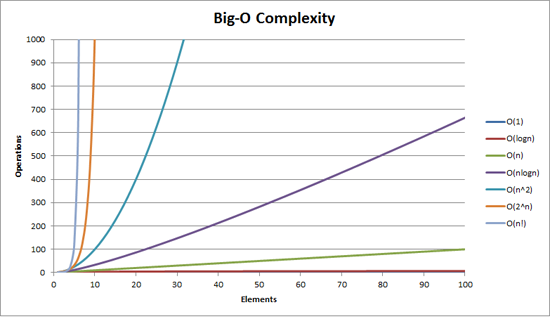
\includegraphics[width=0.7\textwidth]{complexity.png} % <- formatos PNG, JPG e PDF
	\fonte{PERRETT, 2010\nocite{Perrett2010}}
	\label{fig:complexity}
\end{figure}

\section{Programação dinâmica}
\label{sec:pd}

Programação dinâmica é uma técnica que combina soluções de subproblemas, de forma similar à técnica de divisão e conquista, que divide o problema em subproblemas, resolve cada um recursivamente e depois faz a junção das soluções para resolver o problema original. Porém, este método é normalmente utilizado quando os subproblemas se sobrepõem, ou seja, um mesmo estado é encontrado diversas vezes na etapa de divisão. Portanto, se fosse aplicado um Algoritmo ingênuo de divisão e conquista, um mesmo estado seria resolvido várias vezes, aumentando o custo computacional do Algoritmo \cite{Cormen09a}. 

Para resolver o problema de sobreposição, a técnica de programação dinâmica salva a resposta de todos os estados que vão sendo encontrados. Assim, no momento em que se deparar com algo que já foi resolvido ela simplesmente retorna o valor que já estava armazenado. 

A sequência de Fibonacci é um exemplo de fácil entendimento de quando é necessária a utilização de programação dinâmica. Esta é uma sequência de números inteiros que tem seu início com 0 e 1, e os termos subsequentes são uma soma dos dois últimos números. A sequência recebeu o nome do matemático Leonardo de Pisa, mais conhecido como Fibonacci, que no ano de 1202 descreveu o crescimento da população de coelhos utilizando esta sequência \cite{LiveScience2013}. Os primeiros termos são:
\begin{equation}
0, 1, 1, 2, 3, 5, 8, 13, 21, 34, 55, 89, 144, 233, 377, 610, ...
\label{eq:fib}
\end{equation}

A sequência pode ser representada através da seguinte recorrência, onde $fib(i)$ representa $i$-ésimo termo da sequência:
\begin{equation}
fib(i)=
\begin{cases}
i &\text{se } i \leq{1},\\
fib(i - 1) + fib(i - 2) &\text{se } i > {1}.
\end{cases}
\label{eq:fibrecorrence}
\end{equation}

Na Figura \ref{fig:fib5} é apresentada a árvore de recursão gerada ao utilizar a Equação \ref{eq:fibrecorrence} para o cálculo do $fib(5)$. Através dela, é fácil ver que diversos estados estão se repetindo, por exemplo: $fib(2)$ aparece três vezes e sempre que é encontrado ele é divido no $fib(1)$ e $fib(0)$, assim deixando a  complexidade deste Algoritmo em $O(2^{N})$. Ao aplicar programação dinâmica neste Algoritmo é possível reduzir a complexidade para $O(N)$, pois cada estado será expandido uma única vez.

\begin{figure}[H]
	\centering
	\caption[Árvore de recursão do Fibonacci de 5]{Árvore de recursão do Fibonacci de 5}
	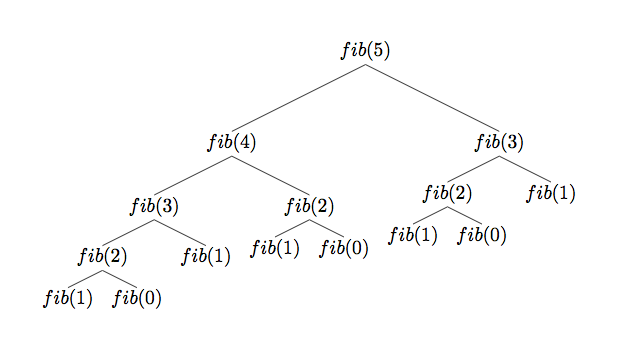
\includegraphics[width=0.7\textwidth]{fib5.png} % <- formatos PNG, JPG e PDF
	\fonte{SCHWARTZ, 2011\nocite{Schwartz2011}}
	\label{fig:fib5}
\end{figure}


O Algoritmo \ref{lst:fibsimples} mostra como seria a implementação da função sem a utilização de programação dinâmica.
\begin{lstlisting}[caption={Implementação Fibonacci sem programação dinâmica em C++},label={lst:fibsimples}]
int fib(int i){
if(i <= 1)
return i;
return fib(i - 1) + fib(i - 2);
}

\end{lstlisting}

Para otimizar o código e utilizar programação dinâmica basta incluir uma tabela que salva todos os estados. Sua inclusão faz uma alteração mínima no código, como é mostrado no Algoritmo \ref{lst:fibpd}.


\begin{lstlisting}[caption={Implementação Fibonacci com programação dinâmica em C++},label={lst:fibpd}]
#define MAX 20 
int tabela[MAX + 1]; 

int fib(int i){
	if(tabela[i] != -1) 
		return tabela[i];
	if(i <= 1)
		return tabela[i] = i;
	return tabela[i] = fib(i - 1) + fib(i - 2);
}
\end{lstlisting}

Para mais informações sobre programação dinâmica e suas técnicas, o site \textit{TopCoder}\footnote{https://www.topcoder.com/community/data-science/data-science-tutorials/} possui um artigo amplo com vários problemas e dicas para soluções. Ele divide sua explicação em teoria e prática, começando nos tópicos mais simples e indo até alguns mais avançados.

\subsection{Otimizações}

Ao utilizar programação dinâmica para otimizar um problema, normalmente ocorre uma queda drástica na classe de complexidade associada à solução, como é o caso da sequência de Fibonacci, discutida na Seção \ref{sec:pd}, onde foi possível sair de uma complexidade exponencial para uma linear. Apesar de parecer uma ótima forma de solucionar um problema, às vezes apenas aplicar programação dinâmica não é suficiente, e existem casos onde é possível e necessário otimizar ainda mais.

Para utilizar uma técnica de otimização de programação dinâmica, alguns critérios em relação à função de recorrência devem ser correspondidos. Cada técnica tem uma abordagem que possibilita a resolução de um conjunto de problemas que compartilham certas propriedades.

A Tabela \ref{tab:otimizacoes} ilustra algumas otimizações existentes, que possibilitam tanto a redução de espaço, quanto de tempo. Estas técnicas serão discutidas no Capítulo \ref{chap:desenvolvimento}.

\begin{table}[H]
	\centering
	\caption[Otimizações de programação dinâmica]{Otimizações de programação dinâmica}
	\label{tab:otimizacoes}
	\begin{tabular}{p{4cm}  p{11cm}}
		\hline \SPACE
		\textbf{Nome/Tipo} & \textbf{Característica} \\ \hline \SPACE
		Redução de espaço &  Reduz a quantidade de memória necessária quando um estado depende de uma quantidade fixa de outros estados \\ \hline \SPACE
		Estrutura de dados &  Reduz a complexidade de tempo com o auxílio de uma estrutura de dados que consegue responder a consultas do tipo mínimo ou máximo em um intervalo de um \textit{array}  \\ \hline \SPACE
		\textit{Divide and Conquer} & Realiza divisão e conquista para encontrar o ponto ótimo necessário para se resolver o estado atual, reduzindo a complexidade temporal \\ \hline \SPACE
		\textit{Knuth Optimization} & Utiliza informações de onde estava a solução ótima de um estado anterior para diminuir o espaço de busca dos outros, assim reduzindo a complexidade temporal  \\ \hline \SPACE
		\textit{Convex Hull Trick} & Através de conceitos geométricos, essa técnica possibilita a redução da complexidade temporal \\ \hline 
	\end{tabular}
	
	\fonte{Pr\'oprio Autor.}
\end{table}

\section{Ensino de Algoritmos}
\label{sec:ensino}

O ensino de Algoritmos, por tratar de assuntos que normalmente não são tão simples, com uma fundamentação matemática extensa, não é uma tarefa fácil. Portanto, foi feita uma busca na literatura de trabalhos que têm por objetivo propor uma metodologia de ensino, servindo de modelo para este trabalho.


\nocite{methods}
Szlávi e Zsakó (2003) apresentaram diversas metodologias relacionadas ao ensino de programação. Os autores discutem sobre alguns modelos e exemplificam quando e para qual nível de estudante cada método será mais proveitoso ao ser aplicado. Estes métodos determinam a forma de estruturar o curso que deseja ser ensinado e a maneira de explicar os conteúdos. Os métodos discutidos no trabalho são:

\vspace{-0.1in}
\begin{itemize}[leftmargin=-.001in]
	\itemsep0em
	\item \textbf{Metodológico, orientado a Algoritmos:} Neste há uma divisão bem clara em todas as etapas do processo de programação, desde a estruturação do que será desenvolvido, até a documentação final. Este é recomendado para ser utilizado com estudantes no final do ensino médio ou que estejam se preparando para um trabalho na área de informática.
	\item \textbf{Orientado a dados}: Este método é similar ao anterior, porém com foco nas estruturas de dados, assim, muitas vezes conseguindo evitar os grandes teoremas que normalmente são complexos e necessários para fazer a explicação dessas estruturas, propondo uma forma mais suave de transmitir o conhecimento.
	\item \textbf{Orientado à especificação:} A especificação da forma que o programa deve funcionar é a parte mais significativa, e todos os Algoritmos são gerados sistematicamente através de rígidas instruções. Método indicado para estudantes universitários de informática, pois este será bem sucedido se os alunos possuírem um profundo conhecimento matemático.
	\item \textbf{Orientado a problemas:} Este método possui grandes diferenças em relação aos outros. Nele toda a etapa de programação é vista como uma única tarefa que não pode ser dividida. Dentre todos os métodos discutidos, este é o único recomendável para todos os tipos de estudantes, pois o foco é desenvolver nos alunos uma forma mais algorítmica de pensar sem estar preocupado com o treinamento profissional.
	\item \textbf{Orientado à linguagem:} Método semelhante ao orientado a problemas, porém o ensino depende totalmente de uma linguagem de programação e todos os ensinamentos são voltados especificamente para a linguagem adotada. Devido a estes fatores esse método está desatualizado e não é tão útil nos dias atuais.
	\item \textbf{Orientado a instruções:} Semelhante ao orientado a linguagem, porém aqui é definida uma linguagem geral, uma forma de pseudocódigo.
	\item \textbf{Orientado à matemática:} Os problemas a serem resolvidos com esta técnica, são retirados da matemática, onde cada problema individualmente é relacionado com algum outro utilizando os princípios básicos da matemática. Esta não é uma metodologia eficaz para o ensino de programação. Porém, o ensino de matemática com o auxílio de programação pode ser útil devido à forma de raciocínio que as duas áreas possuem.
\end{itemize}
\vspace{-0.1in}

\nocite{doi:10.1076/csed.13.2.137.14200} 
No trabalho de Robins e Rountree (2003), uma ampla pesquisa na literatura com o foco na parte educacional do estudo de programação foi feita. Diversos métodos e tópicos foram identificados e analisados para poder ser realizada uma classificação, e assim, auxiliar os professores a identificar em seus alunos características comuns e padrões, que poderão ser contornados com base no que já foi realizado e está documentado na literatura.

\nocite{Pears:2007:SLT:1345443.1345441}
Pears \textit{et al.} (2007) desenvolveu um \textit{survey} que reúne algumas formas da literatura de ensinar introdução à programação. Além disso, os trabalhos reunidos, foram classificados e agrupados pela forma de ensino e pelos métodos aplicados.


\nocite{teachingapplications} 
Zsakó e Nóra (2008) realizaram uma análise dos principais métodos e aplicações que auxiliam no aprendizado e no ensino dos tópicos de\sigla{ICT}{Information and Communication Technology}(do inglês, \textit{Information and Communication Technology}). Para cada método é exemplificado o seu funcionamento, como realizar a sua aplicação e para qual nível de estudante ele é mais apropriado. 


\nocite{teachingapplicationslanguages} 
No trabalho desenvolvido por Papp-varga, Szlávi e Zsakó (2008), foi feita uma análise semelhante à que foi realizada no trabalho apresentado na subseção anterior. Porém, o foco deste é o ensino de uma linguagem de programação, portanto os métodos apresentados demostram os passos ideais para transmitir os conceitos da linguagem proposta.

\nocite{newapproach} 
Radošević, Orehovački e Lovrenčić (2009), propõem a criação de uma ferramenta que facilite o aprendizado de linguagens de programação básicas, como C++, ao invés da utilização de\sigla{IDE}{Integrated Development Environment}(do inglês, \textit{Integrated Development Environment}). A finalidade desta ferramenta é ajudar os estudantes em não cometer erros que são comuns a quem está iniciando e, além disso, permitir ao professor auxiliar seus alunos de forma mais simples.

\nocite{Vihavainen:2011:EAM:1953163.1953196}
Vihavainen, Paksula e Luukkainen (2011), discutem como ensinar o básico de programação para quem está começando. O autor propõe um modelo de ensino e faz a aplicação deste em uma turma de um curso de ciência da computação. O modelo discutido tem três estágios. No primeiro o professor oferece aos estudantes um modelo conceitual de um problema e como o mesmo foi resolvido. A todo momento de explicação o professor verbaliza os seus pensamentos e explica o motivo de ter feito determinada decisão, deixando os alunos acompanharem toda sua linha de raciocínio. Na segunda etapa, o estudante é exposto a um problema que será resolvido com a orientação de um instrutor que não entrega diretamente a resposta, mas sim sugestões que permitam os alunos serem capazes de descobrir as respostas para suas próprias perguntas. A última etapa é quando os alunos conseguem resolver as tarefas sozinhos e não precisam mais do auxilio de um instrutor. Ao final do trabalho é feito um comparativo entre uma turma que utilizou a metodologia proposta e uma que não usou, e os resultados foram positivos, mostrando que as quantidades de evasão e reprovação foram reduzidas.

Apesar de existirem diversos trabalhos que tratam sobre o ensino de Algoritmos e programação, todos os encontrados têm um foco para um nível básico de conhecimento, levando em conta alunos que estão iniciando nesta área. Portanto, não será aplicado nenhum deste diretamente. No Capítulo \ref{chap:metodo} será discutida a metodologia elaborada para a construção do trabalho.





    
\chapter{Trabalhos relacionados}
\label{chap:historico}

Nesta seção são apresentados alguns trabalhos que têm um objetivo similar ao deste projeto. Em todos os encontrados a intenção do autor foi criar um conteúdo teórico sobre algoritmos e programação. Apesar de apenas um trabalho possuir conteúdo relacionado a programação dinâmica, todos eles foram considerados para a elaboração da metologia a ser desenvolvida.

Tommasini (201-) em seu trabalho visa ensinar programação dinâmica para quem está iniciando nesta área. Sua maior motivação foi a falta de um bom material didático sobre esse tema. Seu trabalho tem um foco muito didático, apresentando diversas técnicas, problemas com soluções e propondo vários exercícios para o leitor praticar o que foi ensinado. Ao final do trabalho é apresentada uma lista de problemas de maratonas de programação sobre os assuntos desenvolvidos no texto.


No trabalho proposto por Dalalio (2013), foi realizado um estudo de algoritmos e estruturas de dados para a resolução de problemas relacionados a \textit{String Matching}\footnote{https://en.wikipedia.org/wiki/String\_searching\_algorithm}. Seu texto é bem didático, mostrando diversos problemas e as diversas formas de resolução, apresentando a complexidade e seu código. Ao final diversos problemas são propostos para que o leitor os resolva utilizando os conceitos elaborados no texto.


Couto (2016) desenvolveu um trabalho voltado ao ensino de algoritmos, com foco principal nos algoritmos aplicados em sequências de caracteres. Seu texto está dividido em diversos capítulos, cada um deles apresentando uma estrutura de dados diferente, assim podendo mostrar ao leitor quando é melhor utilizar uma em relação às outras.






    
    
\chapter{Metodologia}
\label{chap:metodo}

Após a análise dos trabalhos levantados no seção \ref{sec:ensino}, pode-se destacar os trabalhos elaborados por Szlávi e Zsakó (2003) e Vihavainen, Paksula e Luukkainen (2011). O primeiro em um dos métodos discutidos é abordado uma forma mais metodológica na hora de transmitir uma informação, onde em cada etapa do ensino há uma clara divisão. No segundo trabalho é mostrado uma maneira de ensino baseada no desenvolvimento de uma linha de raciocínio, em que o aluno ou o leitor, vai acompanhando todos os passos que o instrutor fez até chegar numa conclusão.

A metodologia aplicada no próximo capítulo tomará como base esses dois trabalhos, levando uma linha bem divida entre os tópicos, porém sempre fazendo o leitor entender toda a linha de raciocínio, com algumas pausas a fim de deixar quem está lendo pensar em uma solução para um problema, antes de ser mostrado a resposta, além disso alguns exercícios serão propostos para quem desejar praticar o que está sendo demonstrado.

A estrutura de cada seção será dividida em seis partes, sendo elas:

\begin{itemize}
\item \textbf{Problema:} Será apresentado um problema com todas as informações que são importantes para ser resolvido através de programação dinâmica;
\item \textbf{Solução ingênua:}  A partir da descrição do problema será elaborada uma solução que utilize programação dinâmica , juntamente com a análise de complexidade, podendo ser temporal e/ou de espaço;
\item \textbf{Análise de particularidades:} Após uma solução ter sido desenvolvida será levantado as características do problema, sendo elas a forma que os cálculos estão sendo desenvolvidos, como está sendo armazenado as informações, para que com estes dados possa ser feita alguma otimização. Neste ponto o leitor já começa a imaginar o que pode ser realizado para melhorar a solução;
\item \textbf{“Nome da técnica”:} Com todas as análises feitas, será formulado a técnica em questão, mostrando o seu funcionamento e como esta pode ser aplicada no problema;
\item \textbf{Benefícios:} Tendo aplicado a otimização, uma análise dos benefícios será feita juntamente com as novas complexidades;
\item \textbf{Código final:} Ao final uma forma de implementação do problema com a linguagem C++ será apresentada, com o objetivo de sanar possíveis dúvidas do leitor.
\end{itemize}

Entre cada tópico pode existir algumas paradas com sugestões de tarefas que o leitor pode fazer, para tentar exercitar os conteúdos, estas serão apresentadas conforme o seguinte modelo:

\tikz[baseline=-4pt,align=left]\node[draw,minimum width=12.5cm,minimum height=4ex] {\textit{Sugestão de tarefa ao leitor...}};
    \chapter{Desenvolvimento}
\label{chap:desenvolvimento}
\setcounter{lstlisting}{2}
\setcounter{equation}{2}
Esta seção irá apresentar as técnicas selecionadas de otimização para programação dinâmica, de acordo com a metodologia proposta. Estas serão dividas em subseções, sendo as mesmas independentes entre si.

\section{Redução de espaço}

\begin{itemize}[leftmargin=-.001in]
\item \textbf{Problema:}
 São dados diversos itens, onde cada um possui um peso e valor associado. Deseja-se colocar alguns em uma mochila\footnote{http://www.geeksforgeeks.org/dynamic-programming-set-10-0-1-knapsack-problem/} com a finalidade de maximizar o valor dos que foram selecionados. Porém, a mochila possui uma capacidade máxima de peso. Além disso, nenhum item pode ser fracionado.
\item \textbf{Solução ingênua:} 
\begin{equation}
dp[i][j] = 
\begin{cases}
0 &\text{se } i = 0 \text{ ou } j = 0,\\
max(valor[i-1] + dp[i-1][j-peso[i-1]], dp[i-1][j]) &\text{se } peso[i-1] \leq{j},\\
dp[i-1][j] &\text{se } peso[i-1] > j
\end{cases}
\label{eq:knapsack}
\end{equation}

O problema da mochila pode ser resolvido através da relação de recorrência apresentada acima, onde $dp[i][j]$ representa o valor máximo que pode se conseguir ao colocar os $i$-ésimos primeiros itens em uma mochila de capacidade $j$. Os vetores $valor$ e $peso$, representam o valor e peso associado a cada um dos $n$ itens, respectivamente. A resposta para o problema estará em $dp[n][capacidade]$.


\item \textbf{Análise de particularidades:}
Analisando a complexidade da Equação \ref{eq:knapsack} é fácil ver que será necessário $O(n*capacidade)$, tanto de memória, quanto de tempo. Porém, pode-se perceber que para solucionar a linha $i$ da matriz de programação dinâmica, são necessárias apenas as respostas que já foram calculadas na linha $i - 1$.


\item \textbf{Redução de espaço:} 
Esta técnica visa solucionar problemas onde a quantidade de memória alocada não é sempre necessária, fazendo com que seja mantido em memória apenas o essencial. Para todos os problemas onde uma linha de uma tabela da programação dinâmica dependa de uma quantidade fixa de outras linhas, digamos $K$, é necessário apenas manter em memória $K$ linhas.

No problema proposto, verificou-se que uma linha depende de apenas uma outra. Portanto, podemos trabalhar apenas com duas linhas consecutivas da matriz, sempre alternando entre linha par e ímpar. 
A Equação \ref{eq:knapsackmemorialinear} a seguir demonstra como fazer essa alternância entre linhas:
\begin{equation}
dp[i\&1][j] = \\
\begin{cases}
0 &\text{se } i = 0 \text{ ou } j = 0,\\

max(valor[i-1] + dp[\text{\textasciitilde}i\&1][j-peso[i-1]],\\ dp[\text{\textasciitilde}i\&1][j]) &\text{se } peso[i-1] \leq{j},\\
dp[\text{\textasciitilde}i\&1][j] &\text{se } peso[i-1] > j
\end{cases}
\label{eq:knapsackmemorialinear}
\end{equation}

\tikz[baseline=-4pt,align=left]\node[draw,minimum width=12.5cm,minimum height=4ex]
{\textit{Sugere-se ao leitor tentar utilizar essa técnica na resolução do Fibonacci, que foi} \\\textit{explicado na Seção \ref{sec:pd}}. };
\\
\item \textbf{Benefícios:} 
A Equação \ref{eq:knapsackmemorialinear} ilustra como reduzir a memória. Os valores que serão utilizados nas linhas da tabela de programação dinâmica serão sempre 0 ou 1, assim o total de memória necessária é de $2*capacidade$, deixando com uma complexidade espacial de $O(capacidade)$. Uma maneira simples de alternar entre par e ímpar é utilizar operações binárias. Para verificar se um número é ímpar, basta fazer o \textit{E} entre o número desejado e o número 1, assim o valor retornado será 1 se for ímpar e 0 se for par. Agora para saber a paridade da linha anterior, basta inverter a paridade da linha atual, para isto pode-se usar o operador \text{\textasciitilde}, que é responsável por inverter todos os bits de um número. A resposta para o problema da mochila utilizando esta relação estará em $dp[n\&1][capacidade]$.


\item \textbf{Código final:} 
O Algoritmo \ref{lst:lis} mostra a implementação da solução para o problema da mochila com complexidade de memória linear.
\begin{lstlisting}[caption={Implementação Mochila em C++},label={lst:lis}]

int mochila(){
	int valor[] = {60, 100, 120};
	int peso[]  = {10, 20, 30};
	int capacidade = 50, n = 3;

	int dp[2][capacidade + 1];
	for(int i = 0; i <= n; i++){
		for(int j = 0; j <= capacidade; j++){
			if(!i || !j)
				dp[i&1][j] = 0;
			else if(peso[i - 1] <= j)
				dp[i&1][j] = max(valor[i-1] + dp[~i&1][j-peso[i-1]],
														dp[~i&1][j]);
			else
				dp[i&1][j] = dp[~i&1][j];
		}
	}
	return dp[n&1][capacidade]; 
}
\end{lstlisting}
\end{itemize}


\section{Estrutura de dados RMQ}

\begin{itemize}[leftmargin=-.001in]
 \item \textbf{Problema:} Um dos problemas clássicos de programação dinâmica é a\sigla{LIS}{Longest Increasing Subsequence}(do inglês, \textit{Longest Increasing Subsequence})\footnote{http://www.geeksforgeeks.org/longest-increasing-subsequence/}. Neste, o objetivo é encontrar a maior subsequência de um \textit{array} onde todos os elementos estão ordenados de forma crescente. Uma subsequência pode ser encontrada com a eliminação de alguns elementos do \textit{array}.

Imaginemos o seguinte \textit{array}:

\begin{center}
	${2, 5, 3, 7, 11, 8}$
\end{center}

Uma das soluções para este conjunto é a subsequência ${2, 3, 7, 8}$, que possui tamanho quatro, porém esta não é única, existem outras com o mesmo tamanho, como é o caso da subsequência ${2, 5, 7, 11}$. Geralmente é esperado apenas o tamanho da maior LIS possível. Portanto, qual LIS será escolhida não terá muita relevância, pois só será necessário se preocupar com isso quando houver a necessidade da reconstrução da solução.

\item \textbf{Solução ingênua:} Este problema pode ser facilmente resolvido com o auxilio de programação dinâmica utilizando a seguinte recorrência:

\begin{equation}
dp[i] = 
\begin{cases}
1 &\text{se } i = 0 \\
max(dp[j] + 1)_{0 \leq j < i} &\text{se } i \neq 0 \text{ e } v[j] \leq v[i]

\end{cases}
\label{eq:lisQuadrado}
\end{equation}

A Equação \ref{eq:lisQuadrado}, resolve o problema da LIS, com a complexidade $O(n^2)$ de tempo e $O(n)$ de memória. Nesta solução, $dp[i]$ representa qual a maior LIS que pode ser formada onde o último elemento é exatamente o índice $i$. Para calcular cada estado $i$ é selecionado um estado $j$ que já tenha sido calculado e possui maior valor. Além disso, o valor do elemento $j$ tem que ser menor ou igual que o elemento $i$. Isto significa que a LIS que termina em $i$ é uma junção da LIS terminada em $j$, adicionado o elemento $i$ ao final dela. Após calcular todos os estados utilizando a recorrência, basta percorrer o $array$ $dp$ e obter seu maior valor.

\item \textbf{Análise de particularidades:} É notório que quando está sendo calculada a $dp[i]$, ou seja, a maior LIS que termina no $i$-ésimo índice, estão sendo percorridos todos elementos do $array$ que estão à esquerda e que possuem um valor menor ou igual que o elemento atual. Em outras palavras, queremos o maior elemento da $dp$ cujo valor esteja no intervalo $[0..v[i]]$.
\\

\tikz[baseline=-4pt,align=left]\node[draw,minimum width=12.5cm,minimum height=4ex]
{\textit{Sugere-se ao leitor pensar uma maneira mais eficiente de encontrar o maior} \\\textit{elemento do array}. };
\\

\item \textbf{Estruturas de dados RMQ:}
Existem algumas estruturas de dados que resolvem problemas parecidos com este, onde é dado um \textit{array} e é necessário consultar o máximo ou mínimo elemento em um determinado intervalo. Essas operações normalmente são chamadas de\sigla{RMQ}{Range Minimum Query}(do inglês, \textit{Range Minimum/Maximum Query}). Espera-se destas estruturas uma complexidade melhor que $O(n)$, que seria a forma mais simples de conseguir o máximo, bastando apenas iterar por todo o intervalo. É o 
caso da $Segment Tree$\footnote{http://www.geeksforgeeks.org/segment-tree-set-1-range-minimum-query/} ou $BIT$\footnote{http://www.geeksforgeeks.org/binary-indexed-tree-or-fenwick-tree-2/}, que realizam estas operações em $O(logn)$.

\item \textbf{Benefícios:} Ao remover a busca linear para encontrar o maior elemento já calculado, adicionando uma das estruturas citadas, a complexidade da busca será reduzida de $O(n)$ para $O(logn)$, deixando assim a LIS em uma complexidade final de $O(n*logn)$.

\item \textbf{Código final:} 
O Algoritmo \ref{lst:lis} mostra uma maneira de implementar a solução para a LIS utilizando $BIT$.
\begin{lstlisting}[caption={Implementação LIS em C++},label={lst:lis}]

#define MAXN 20
int v[] = {2, 5, 3, 7, 11, 8};
int bit[MAXN];
int dp[MAXN];

void update(int x, int v){
	for(; x < MAXN; x+=x&-x)
		bit[x] = max(bit[x], v);
}

int get(int x){
	int ans = 0;
	for(; x; x-=x&-x)
		ans = max(ans, bit[x]);
	return ans;
}

int lis(int n){
	int ans = 0;
	
	for(int i = 0; i < n; i++){
		dp[i] = 1+get(v[i]);
		update(v[i], dp[i]);
		ans = max(ans, dp[i]);
	}
	
	return ans;
}
\end{lstlisting}
\end{itemize}
\section{\textit{Divide and Conquer Optimization}}
\begin{itemize}[leftmargin=-.001in]
\item \textbf{Problema:}
São dados $n$ objetos, cada um com um valor associado $x_{1}, x_{2}, x_{3}, ..., x_{n}$, onde $x_{i} > 0$ $_{\forall{i}}$ e é necessário dividi-los em $k$ grupos consecutivos, de forma que esta divisão seja feita com o menor custo possível. O custo para criação de um grupo é igual à soma dos valores de todos elementos do grupo multiplicado pela quantidade de objetos.

Para exemplificar, supondo que são quatro objetos e seus valores são {1, 2, 3 e 4}, é necessário dividi-los em dois grupos. Uma divisão possível seria colocar os objetos com valores {1, 2, 3} no primeiro grupo o que resultaria em um custo de 18, ou seja, a soma deles que é igual a 6, multiplicado pela quantidade de elementos, 3. Por fim, o elemento 4 ficaria no segundo grupo, tendo como custo o valor 4. Portanto para esta configuração o custo total é a soma dos dois grupos, o que gera um valor de $18+4=22$. Analisando um pouco melhor este exemplo é fácil notar que esta configuração não é a melhor possível. A solução ótima seria deixar os objetos com valores 1 e 2 no primeiro grupo e os demais elementos no segundo grupo, gerando um custo total de 20.

\item \textbf{Solução ingênua:} Para resolver este problema, o primeiro passo é calcular uma matriz $C[i][j]$, que corresponde ao custo total para agrupar todos os elementos do índice $i$ até o índice $j$. O tempo total para calcular a matriz poderá ser de ordem quadrática.
\\

\tikz[baseline=-4pt,align=left]\node[draw,minimum width=12.5cm,minimum height=4ex]
{\textit{Fica como sugestão ao leitor implementar o cálculo da matriz $C$ com tempo $O(n^2)$.}};
\\

A Equação \ref{eq:dc1} exemplifica uma maneira de implementar o problema, onde $dp[i][j]$ representa o menor custo para criar $i$ grupos estando no $j$-ésimo objeto. A resposta estará em $dp[k][n]$, levando em consideração que o $array$ está indexado a partir da posição 1. Para solucionar cada estado é necessário percorrer todos os elementos que são menores que $j$ e verificar se criar um novo grupo naquela posição irá melhorar solução. Para tal, serão feitas em média $n/2$ iterações, o que leva a uma complexidade final de $O(k*n^2)$.

\begin{equation}
dp[i][j] =
\begin{cases}
0 &\text{se } i = 0 \\
C[i][j] &\text{se } i = 1 \\
min_{l < j}(dp[i-1][l] + C[l+1][j]) &\text{se } i > 1
\end{cases}
\label{eq:dc1}
\end{equation}

\item \textbf{Análise de particularidades:} 
Se for definida uma matriz $opt[i][j]$ que representa qual é o $l$ ótimo para realizar a divisão da $dp[i][j]$, ou seja, o ponto ótimo que minimiza o valor daquele estado, é possível notar que para qualquer $i$ e $j$, $opt[i][j] \leq opt[i][j+1]$. Portanto, $j$ é monotônico\footnote{https://en.wikipedia.org/wiki/Monotonic\_function} para um $i$ fixo. Isto é verdade pois ao inserir um novo objeto em um grupo o valor deste só poderá aumentar, devido à formulação da função de custo. Assim, um conjunto com $x+1$ elementos não poderá ter um ponto ótimo de divisão menor do que este mesmo conjunto com $x$ elementos.

\item \textbf{\textit{Divide and Conquer Optimization}:} Devido à monotonicidade de $opt$, pode-se melhorar a complexidade da solução proposta, pois, como observado, para calcular o estado ($i$, $j+1$), não é necessário testar valores de $l$ que são menores do que $opt[i][j]$, apenas valores que são maiores ou iguais a $opt[i][j]$. Para a implementação desta técnica podemos recorrer à divisão e conquista\footnote{https://pt.wikipedia.org/wiki/Divisão\_e\_conquista}, onde pode-se criar uma função recursiva. Para um $i$ fixo, é aplicada a divisão e conquista no $j$, sendo mantido o intervalo do $j$ e o intervalo válido de $l$, que representa o ponto ótimo.

\item \textbf{Benefícios:} Ao calcular o valor e o ponto ótimo $x$ para um estado $j$, a divisão em conquista se responsabilizará por chamar a recursão para resolver o estado $j-1$ com o intervalo de $l$ variando de $1..x$ e a recursão para o estado $j+1$ com o $l$ entre $x..n$. Assim, é perceptível que o intervalo de busca do ponto ótimo que no início era $1..n$, foi dividido pela metade, e este é exatamente o pior caso, quando o ponto ótimo está exatamente no meio. Portanto, para calcular um estado $j$ para um $i$ fixo, a complexidade é $O(n*logn)$, bem menor do que a solução ingênua que gastava $O(n^2)$ para cada $i$. Sendo assim, a complexidade final ao aplicar esta técnica neste problema fica $O(k*n*logn)$.
\item \textbf{Código final:} O Algoritmo \ref{lst:dc} é apresenta um código que resolve este problema. Para obter a solução basta chamar a função $divideAndConquer()$, passando como parâmetro o total de elementos e a quantidade de grupos desejados.
\\

\tikz[baseline=-4pt,align=left]\node[draw,minimum width=12.5cm,minimum height=4ex]
{\textit{Fica como sugestão ao leitor resolver o problema 2475 - Confecção de Presentes} \\\textit{do site URI - Online Judge}};

\begin{lstlisting}[caption={Implementação Divide and Conquer em C++},label={lst:dc}]
#define MAXN 10
#define inf 99999999
int arr[MAXN] = {1, 2, 3, 4};
int C[MAXN][MAXN], dp[MAXN][MAXN];

void solve(int i, int jInicio, int jFim, int optInicio, int optFim){
	if(jInicio > jFim) return;	
	int mid = (jInicio + jFim) / 2;
	dp[i][mid] = inf;
	int opt = -1;
	
	for(int l = optInicio; l <= min(optFim, mid); l++){
		if(dp[i-1][l] + C[l+1][mid] < dp[i][mid]){
			dp[i][mid] = dp[i-1][l] + C[l+1][mid];
			opt = l;
		}
	}	
	solve(i, jInicio, mid-1, optInicio, opt);
	solve(i, mid+1, jFim, opt, optFim);
}

int divideAndConquer(int n, int k){
	// Calculo da funcao custo O(n^2)
	for(int i = 0; i < n; i++){
		int soma = 0;
		for(int j = i; j < n; j++){
			soma += arr[j];
			C[i][j] = soma*(j-i+1);
		}
	}	
	// Casos base
	for(int i = 0; i < n; i++)
		dp[0][i] = 0;
	for(int i = 0; i < n; i++)
		dp[1][i] = C[0][i];
	
	for(int i = 2; i <= k; i++)
		solve(i, 0, n-1, 0, n-1);
	
	return dp[k][n-1];
}

\end{lstlisting}
\end{itemize}
\section{\textit{Knuth Optimization}}
\begin{itemize}[leftmargin=-.001in]
\item \textbf{Problema:}
Uma \textit{string} é dada e deseja-se realizar alguns cortes nela. A cada corte feito, ela será dividida em duas partes e haverá um custo associado para fazer tal operação, que é igual exatamente ao tamanho original antes de efetuar o corte. Imaginemos a \textit{string} \enquote{knuthoptimization} que possui $17$ caracteres e é preciso realizar os cortes nos índices 2, 6 e 8, levando em consideração que a \textit{string} está indexada começando em $1$.
O valor total para realizar todos os cortes, está diretamente relacionado à ordem escolhida para efetuar as divisões. As Tabelas \ref{tab:knuthCorte} e \ref{tab:knuthCorte2} mostram os custos associados ao realizar os cortes de duas maneiras distintas. Na Tabela \ref{tab:knuthCorte} os cortes foram feitos da esquerda para a direita, enquanto a Tabela \ref{tab:knuthCorte2} mostra como ficaria a resposta se os cortes fossem feitos da direita para a esquerda.

\begin{table}[H]
	\centering
	\caption[Problema Knuth realizando cortes da esquerda para a direita]{Problema Knuth realizando cortes da esquerda para a direita}
	\label{tab:knuthCorte}
	\begin{tabular}{p{3cm}p{4cm}p{3cm}}
		\hline \SPACE
		\textbf{Corte} & \textbf{\textit{String}} & \textbf{Custo} \\  \hline \SPACE
		- & knuthoptimization    &  0\\ \hline \SPACE
		2 & kn uthoptimization   &  17\\ \hline \SPACE
		6 & kn utho ptimization  &  15\\ \hline \SPACE
		8 & kn utho pt imization &  11\\ \hline \SPACE
		\textbf{Total}  & -   &  43 \\ \hline  
	\end{tabular} 	
\end{table}
\fonte{Pr\'oprio Autor.}

\begin{table}[H]
	\centering
	\caption[Problema Knuth realizando cortes da direita para a esquerda]{Problema Knuth realizando cortes da direita para a esquerda}
	\label{tab:knuthCorte2}
	\begin{tabular}{p{3cm}p{4cm}p{3cm}}
		\hline \SPACE
		\textbf{Corte} & \textbf{\textit{String}} & \textbf{Custo} \\  \hline \SPACE
		- & knuthoptimization    &  0\\ \hline \SPACE
		8 & knuthopt imization   &  17\\ \hline \SPACE
		6 & knutho pt imization  &  8\\ \hline \SPACE
		2 & kn utho pt imization &  6\\ \hline \SPACE
		\textbf{Total}  & -   &  31 \\ \hline  
	\end{tabular} 	
\end{table}
\fonte{Pr\'oprio Autor.}

Ao analisar as tabelas, fica evidente que a ordem do corte fará com que o custo total aumente ou diminua. O problema consiste em determinar qual é o menor valor possível para realizar todas as divisões propostas.
\\

\tikz[baseline=-4pt,align=left]\node[draw,minimum width=12.5cm,minimum height=4ex]
{\textit{Para melhor entendimento, é sugerido ao leitor encontrar o menor custo para} \\\textit{o exemplo proposto.}};
\\

\item \textbf{Solução ingênua:} Para resolução deste problema, a primeira coisa importante a se notar é que o tamanho da \textit{string} não é tão importante. O mais relevante é onde os cortes devem ser realizados. Assim, as complexidades das soluções estarão ligadas à quantidade \textit{k} de cortes.

Sendo o \textit{array} $v_{1}, v_{2}, ..., v_{k}$ representando as posições de cada divisão, onde $v_{1} < v_{2} < ... < v_{k}$, pode ser pensado em uma solução com programação dinâmica que utilize dois ponteiros, $i$ e $j$, que representam quais posições estão sendo analisadas no momento. Para solucionar cada estado basta escolher uma posição $x$ onde $i < x < j$, que minimize o custo.

\begin{equation}
dp[i][j] =
\begin{cases}
0 &\text{se } j-i \leq 1 \\
min_{i < x < j}(dp[i][x] + dp[x][j] + v[j] - v[i]) &\text{se } j-i > 1
\end{cases}
\label{eq:knuthBruto}
\end{equation}

A Equação \ref{eq:knuthBruto} apresenta uma possível solução para o problema, onde o custo para realizar um corte está representado como sendo $v[j]-v[i]$, ou seja, o tamanho da \textit{string} que está sendo considerada. Porém, através da definição do problema, é sabido que para realizar o primeiro corte o custo será igual ao tamanho original da \textit{string}, mas esta solução não está tratando esse caso. Uma solução simples é inserir dois elementos extras no \textit{array} de cortes, que irão representar o tamanho completo. Após essa modificação, este terá o formato $v_{0}, v_{1}, v_{2}, ..., v_{k}, v_{k+1}$, onde $v_{0}$ tem o valor $0$ e $v_{k+1}$ possui o tamanho inteiro da \textit{string}. Com estas modificações o algoritmo proposto irá funcionar e a resposta estará em $dp[0][k]$.
Para solucionar cada estado $(i, j)$ da matriz, é necessário iterar por todos elementos que estão neste intervalo para encontrar o melhor candidato à resposta. Por conta disso a complexidade final será $O(k^3)$.

\item \textbf{Análise de particularidades:}
Se for definida uma função de custo $C[i][j]$ que representa o valor para cortar um \textit{string} estando nos índices $i$ e $j$ do \textit{array} $v$, esta pode ser interpretada como sendo $C[i][j] = v[j]-v[i]$. É possível notar que o custo é monotônico, respeitando a Equação \ref{eq:monotonicidadeKnuth}.
\begin{equation}
C[b][c] \leq C[a][d] , a \leq b \leq c \leq d
\label{eq:monotonicidadeKnuth}
\end{equation}

Essa equação implica que todos os subintervalos possuem um custo menor ou igual ao intervalo onde o mesmo está contido. Para melhor entendimento, pode-se imaginar o seguinte \textit{array} de cortes, com os índices variando de 1 até 5: $v = \{1, 2, 5, 10, 15\}$. Se como intervalo maior forem selecionados os elementos nas posições 1 e 5, o custo será 14. Porém, ao selecionar duas posições $x$ e $y$, onde $1 \leq x \leq y \leq 5$ é evidente que não será possível ter um custo maior que 14.
\\

\tikz[baseline=-4pt,align=left]\node[draw,minimum width=12.5cm,minimum height=4ex]
{\textit{Sugere-se ao leitor avançar para a próxima parte da otimização apenas quando o} \\\textit{mesmo tiver compreendido a condição de monotonicidade do problema.}};
\\

\item \textbf{\textit{Knuth Optimization}:} 
Devido à monotonicidade da função de custo, é possível definir uma matriz $opt[i][j]$ que representa qual o menor $x$ que gera a melhor solução para a $dp[i][j]$, ou seja, o ponto ótimo para realizar o corte. É possível notar que para qualquer par de $i$ e $j$, onde $i \leq j$, a propriedade mostrada na Equação \ref{eq:optKnuth} é mantida.

\begin{equation}
opt[i][j-1] \leq opt[i][j] \leq opt[i+1][j]
\label{eq:optKnuth}
\end{equation}

Para melhor entendimento, a equação pode ser dividida em duas partes: na primeira, $opt[i][j-1] \leq opt[i][j]$, fica fácil ver que esta é verdade pois se fixarmos o $i$ e aumentarmos o tamanho do intervalo em 1 para a direita, o ponto ótimo não poderá estar antes do intervalo menor. Isso se deve ao fato do custo ser monotônico. Assim, se fosse melhor realizar o corte na posição $x$ para $i$ e $j$, então para $i$ e $j-1$ também seria ótimo escolher a posição $x$, ou então uma posição menor. O mesmo raciocínio vale para a segunda parte da equação, $opt[i][j] \leq opt[i+1][j]$, porém aqui o intervalo está sendo diminuído em 1.
Baseado nessas características, agora é possível mudar a forma de calcular o valor de $x$ da Equação \ref{eq:knuthBruto}, fazendo com que ele itere apenas entre $opt[i][j-1]$ e $opt[i+1][j]$.

\item \textbf{Benefícios:}
O grande gargalo da solução proposta era o cálculo do ponto ótimo $x$ de cada estado, que em média gastará $O(k)$. Ao utilizar as informações referentes ao $opt$, pode-se calcular a matriz $dp$ em ordem crescente de $j-i$, ou seja, dos menores intervalos até os maiores. Além disso, o $x$ não irá mais variar entre $i+1$ e $j-1$, mas sim entre $opt[i][j-1]$ e $opt[i+1][j]$. Portanto, agora para o cálculo de um estado de tamanho $y = j-i$, o tempo necessário é igual a $opt[y+1][2] - opt[y][1] + opt[y+2][3] - opt[y+1][2] + ... + opt[k][k-y+1] - opt[k-1][k-y] = opt[k][k-d+1] - opt[k][1] = O(k)$. Sendo assim, o tempo total para resolver toda a matriz $dp$ sai de $O(k^3)$ para $O(k^2)$.
\item \textbf{Código final:} O Algoritmo \ref{lst:knuth} apresenta uma implementação da solução do problema. Para obter a resposta, basta preencher o \textit{array} $v$ com os cortes necessários. Estes deverão estar com os índices entre $1...k$. Ao chamar a função $knuthOptimization()$, passando como parâmetro o tamanho da \textit{string} e o total de cortes, será devolvido o custo mínimo.
\\

\tikz[baseline=-4pt,align=left]\node[draw,minimum width=12.5cm,minimum height=4ex]
{\textit{Fica como sugestão ao leitor resolver o problema BRKSTRNG - Breaking String} \\\textit{do site SPOJ.com}};
\newpage
\begin{lstlisting}[caption={Implementação Knuth Optimization em C++},label={lst:knuth}]
#define MAXN 1010
#define inf 99999999

int v[MAXN];
int dp[MAXN][MAXN];
int opt[MAXN][MAXN];

int knuthOptimization(int n, int k){
	// Adicionado os elementos extras
	v[0] = 0;
	v[++k] = n;
	k++;
	
	for(int tam = 1; tam <= k; tam++){
		for(int i = 0; i+tam <= k; i++){
			int j = i+tam-1;
			if(tam <= 2){
				dp[i][j] = 0;
				opt[i][j] = i;
				continue;
			}
			dp[i][j] = inf;
			for(int x = opt[i][j-1]; x <= opt[i+1][j]; x++){
				if(dp[i][x] + dp[x][j] + v[j]-v[i] < dp[i][j]){
					dp[i][j] = dp[i][x] + dp[x][j] + v[j]-v[i];
					opt[i][j] = x;
				}
			}
		}
	}
	return dp[0][k-1];
}
\end{lstlisting}

\end{itemize}

\newpage
\section{\textit{Convex Hull Trick}}
\begin{itemize}[leftmargin=-.001in]
\item \textbf{Problema:}
Uma estrada está sendo construída e é necessário cobrir $n$ pontos da mesma. O custo para se cobrir um pedaço da estrada que vai do ponto $x$ até o ponto $y$, é definido como $(x-y)^2 + c$, sendo $c$ uma constante qualquer. Para exemplificar, vamos supor o \textit{array} $v = \{1, 3, 8, 10\}$, que representa os pontos que precisam de cobertura, além disso, o valor da constante $c$ é 5. Portanto, uma solução possível seria realizar a cobertura do ponto 1 até o 8, com o custo de $(1-8)^2 + 5 = 54$ e uma cobertura única no ponto 10, totalizando $(10-10)^2 + 5 = 5$. Para tal configuração, o valor total para cobrir os 4 pontos seria de 59. O objetivo deste problema é encontrar o custo mínimo para realizar a cobertura.
\\

\tikz[baseline=-4pt,align=left]\node[draw,minimum width=12.5cm,minimum height=4ex]
{\textit{Para melhor entendimento, é sugerido ao leitor encontrar a melhor solução para} \\\textit{o exemplo proposto.}};
\\

\item \textbf{Solução ingênua:} 
Assumindo que os elementos no \textit{array} $v$, estão indexados em 1, a Equação \ref{eq:chtBruto} mostra uma possível solução.

\begin{equation}
dp[i] =
\begin{cases}
0 &\text{se } i = 0 \\
min_{1 \leq j \leq i}(dp[j-1] + (v[i] - v[j])^2 + c) &\text{se } i \neq 0
\end{cases}
\label{eq:chtBruto}
\end{equation}

Para o cálculo de cada estado $i$ da tabela, é necessário percorrer todos os índices que estão à sua esquerda, com a finalidade de escolher algum ponto onde seria colocado o início da cobertura. Devido a isto, a complexidade de cada estado seria $O(n)$ e a complexidade para o cálculo de todos os $n$ estados seria $O(n^2)$. A solução para o problema estará em $dp[n]$. 

\item \textbf{Análise de particularidades:}
Através do código ingênuo elaborado, pode-se notar que um dos motivos da solução não ficar tão rápida, é o fato de que, para resolver cada estado é necessário percorrer todos os outros que possuem um índice menor. Porém, ao expandir a equação de custo de cada estado, algumas propriedades importantes podem ser notadas. Sua expansão tem a seguinte forma:
$dp[j-1] + (v[i] - v[j])^2 + c = -2*v[j]*v[i] + v[j]^2 + dp[j-1] + v[i]^2 + c$. Para melhor clareza será substituído $v[i]$ por $x$ e $v[j]$ por $y$, assim resultando em:
$-2*y*x + y^2 + dp[j-1] + x^2 + c$. Além disso, se for definido que $a = -2*y$ e $b = y^2 + dp[j-1]$, é possível verificar que para o cálculo de um estado $i$, a iteração que é necessária para encontrar o mínimo, está tentando exatamente minimizar a função $f(x) = ax + b$, que pode ser vista graficamente como uma reta, pois os valores de $x$ são apenas inteiros positivos. A $f(x)$ não contempla os valores de $x^2$ e $c$, pois estes serão somados para qualquer reta selecionada. Logo, não há necessidade de tentar minimizá-los.

\item \textbf{\textit{Convex Hull Trick}:}
Imaginemos que diversas equações lineares sejam dadas, sendo no formato $f(x) = ax + b$, e diversas consultas são efetuadas, onde para cada uma delas é necessário informar qual o menor valor que uma $f(x)$ possui para um determinado $x$ se este for avaliado para todas as equações\footnote{https://wcipeg.com/wiki/Convex\_hull\_trick}. 
Como exemplo imaginemos quatro funções, $f(x) = 4$, $f(x) = \frac{4}{3} + \frac{2}{3}x$, $f(x) = 12 - 3x$ e $f(x) = 3 - \frac{1}{2}x$ e é desejável descobrir qual destas minimiza o valor de $x = 1$. A Figura \ref{fig:chtplot} mostra graficamente a distribuição destas equações que podem ser vistas como restas no plano.

\begin{figure}[H]
	\centering
	\caption[Equações lineares graficamente]{Equações lineares graficamente}
	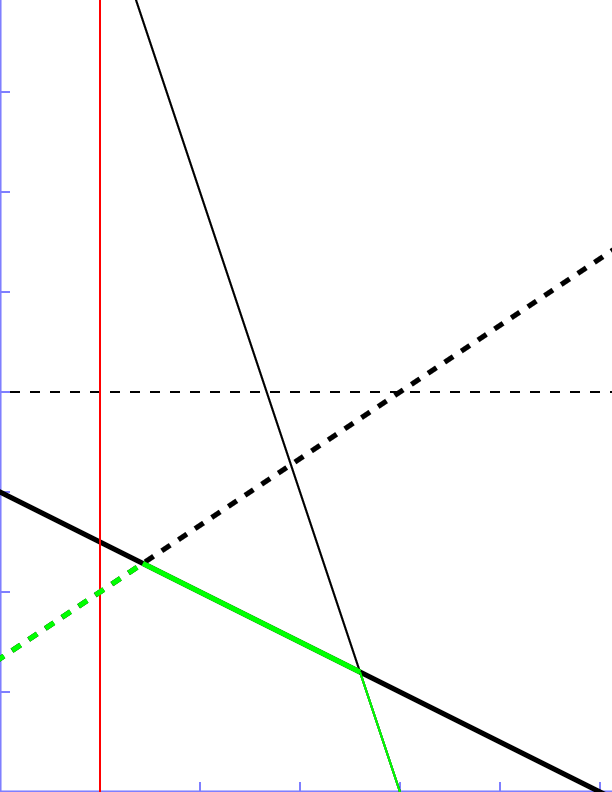
\includegraphics[width=0.5\textwidth]{chtPlot.png} % <- formatos PNG, JPG e PDF
	\label{fig:chtplot}
\end{figure}
\fonte{PEGWIKI, 2016\nocite{Wcipeg2016}}

Para consultar o valor de $x = 1$, que está representado no gráfico acima através da linha vermelha, é possível ver que a reta que gera o menor valor possível é a que está pontilhada com traços grossos, sendo esta a $f(x) = \frac{4}{3} + \frac{2}{3}x$. Analisando esta figura, algumas características importantes podem ser observadas, como é o caso da reta $f(x) = 4$, que claramente nunca será escolhida, independente do valor de $x$, pois sempre haverá alguma outra que possui um valor menor. Dentre as outras três retas, é possível ver que elas são importantes, pois para algum valor de $x$ elas possuem o menor valor de $f(x)$. Isso pode ser visto como a parte em verde pintada nas retas, a qual mostra o intervalo de valores de $x$ onde cada reta é a melhor escolha.
Com a informação de até que ponto uma determinada reta é ótima, elas podem ser ordenadas e cada consulta pode ser resolvida através de uma busca binária\footnote{http://www.geeksforgeeks.org/binary-search/}, onde para cada momento um valor é testado e decidido se a reta ótima para o $x$ em questão está à direita ou à esquerda desta. Assim, cada consulta teria a complexidade $O(log n)$, sendo $n$ o total de retas.

Uma forma de resolver seria adicionar todas as retas em alguma estrutura de dados, ordená-las pela angulação e depois realizar as consultas. Porém, nem sempre as retas estão disponíveis de antemão. Logo, se utilizarmos a ideia de sempre que adicionar uma nova reta for necessário ordenar todas elas, o algoritmo ficaria com a complexidade $O(n^2*log n)$.
\\

\tikz[baseline=-4pt,align=left]\node[draw,minimum width=12.5cm,minimum height=4ex]
{\textit{Sugere-se ao leitor pensar em uma maneira mais eficaz de adicionar uma nova reta} \\\textit{no conjunto.}};
\\

Partindo do princípio que o conjunto de retas está devidamente ordenado e é necessário inserir mais uma reta com angulação maior que as já presentes, ao realizar essa operação alguns casos podem acontecer:
\begin{itemize}
\item A nova reta não é melhor que nenhuma outra que já estava presente, sendo assim, não há necessidade de incluir a mesma no conjunto; 

\item A nova reta é melhor do que algumas outras a partir de algum valor de $x$;

\item A nova reta é melhor que alguma reta em todos os pontos onde esta era ótima, portanto, não é necessário mais manter aquela reta.
\end{itemize}

Com esses casos, um algoritmo mais eficiente pode ser pensado, onde será mantida uma pilha\footnote{http://www.geeksforgeeks.org/stack-data-structure/}, com todas as retas que ainda são ótimas em algum ponto, contendo em seu topo a última que foi adicionada. Quando for inserida uma nova reta, basta verificar se a que estava no topo ainda será útil. Caso seja, a nova reta é inserida, mas se não for, pode-se realizar um $pop()$ da pilha e ir repetindo este passo até que a pilha esteja vazia, ou que uma reta que ainda é útil for encontrada.

Para determinar o momento em que uma reta não é mais relevante e precisa ser removida da pilha, basta verificar se o ponto de intersecção da reta que está sendo inserida no momento com a penúltima reta está à esquerda do ponto de intersecção entre a penúltima e a última reta incluída. Caso isto ocorra, a última reta pode ser removida, pois a partir de agora ela se torna irrelevante. Com essas propriedades é notório que cada reta pode ser adicionada ou removida apenas uma vez, deixando assim a complexidade total $O(n)$ para incluir todas elas.

Esta técnica possui algumas variações e pode-se destacar três delas:

\textit{\textbf{Convex Hull Trick 1:}}  Nesta versão, as consultas realizadas são feitas de maneira crescente, ou seja, $x_{1} \leq x_{2} \leq ... \leq x_{n}$, portanto, pode ser mantido um ponteiro $p_{i}$, que informa em qual reta estava a resposta para a consulta $x_{i}$. Assim, quando for necessário descobrir a resposta para a consulta $x_{i+1}$, só é necessário verificar as retas a partir do $p_{i} + 1$. Pois, no momento que para alguma consulta uma reta não for a melhor, é impossível ela se tornar ótima em algum outro momento. Além disso, todas as retas serão inseridas de maneira ordenada. Isso faz com que todas as consultas sejam respondidas em $O(q + n)$, onde $q$ é o número de consultas e $n$ é o total de retas. Isso se deve ao fato de que cada reta será avaliada apenas uma vez.

\textit{\textbf{Convex Hull Trick 2:}} Esta variação é similar à primeira, porém, as consultas não estão ordenadas. Assim, se faz necessário o uso da busca binária, deixando a complexidade em $O(q*log n)$.

\textit{\textbf{Convex Hull Trick 3:}} Nesta versão não há garantias que as retas serão inseridas de forma ordenada. Assim, a solução proposta utilizando pilha não funciona mais, sendo necessário utilizar outra estrutura de dados. Com o intuito de deixar a complexidade o mais baixa possível, pode ser utilizada uma árvore balanceada para manter as retas ordenadas.
\\

\tikz[baseline=-4pt,align=left]\node[draw,minimum width=12.5cm,minimum height=4ex]
{\textit{Fica como sugestão ao leitor pensar em uma maneira de resolver esta variação.}};
\\


\item \textbf{Benefícios:}
Como visto na etapa de análise de particularidades, as funções de custo possuem a forma $f(x) = ax + b$, logo podem ser descritas como retas, permitindo a aplicação desta técnica. Como pode ser notado, para resolver o estado $i$, só as retas menores que $i$ são importantes. Assim, pode ser inserida a reta relacionada a este estado no momento em que ele for resolvido. Devido a solução ingênua elaborada e a ordenação do \textit{array} $v$, é possível ver que as retas inseridas e as consultas realizadas serão feitas de maneira ordenada. Portanto, pode ser utilizada a variação 1 do \textit{Convex Hull Trick}. Ao aplicar a otimização, a complexidade será reduzida para $O(n + n) = O(n)$.
\item \textbf{Código final:}
O Algoritmo \ref{lst:cht} apresenta a implementação da solução para o problema. Para obter a resposta basta preencher o \textit{array v} com as posições que necessitam de cobertura. Este deverá estar com índices entre $1...n$. Ao chamar a função $cht()$, passando como parâmetro a quantidade de elementos e a constante, será devolvido o custo mínimo para realizar a cobertura de todos os pontos.
\\

\tikz[baseline=-4pt,align=left]\node[draw,minimum width=12.5cm,minimum height=4ex]
{\textit{Fica como sugestão ao leitor resolver o problema Covered Walkway} \\\textit{do site Kattis.com}};
\newpage
\begin{lstlisting}[caption={Implementação Convex Hull Trick 1 em C++},label={lst:cht}]
#define MAXN 10
#define inf 99999999
int v[MAXN] = {0, 1, 3, 8, 10};
int dp[MAXN];
int A[MAXN], B[MAXN];
int tam, ponteiro;

int quadrado(int x){ return x*x; }

void adicionarReta(int a, int b){
	while(tam >= 2 && 
			(B[tam-2] - B[tam-1]) * (a-A[tam-1]) >=
			 (B[tam-1]-b) * (A[tam-1]-A[tam-2]))
		tam--;
	A[tam] = a;
	B[tam] = b;
	tam++;
}

int consultar(int x){
	ponteiro = min(ponteiro, tam-1);
	while(ponteiro+1 < tam && 
		A[ponteiro+1]*x+B[ponteiro+1] <= A[ponteiro]*x + B[ponteiro])
		ponteiro++;
	return A[ponteiro]*x + B[ponteiro];
}

int cht(int n, int c){
	// Inicializando a pilha do Convex Hull Trick
	ponteiro = tam = 0;
	
	// Caso base
	dp[0] = 0;
	adicionarReta(-2*v[1], quadrado(v[1]));
	for(int i = 1; i <= n; i++){
		dp[i] = consultar(v[i]) + quadrado(v[i]) + c;
		if(i < n)
			adicionarReta(-2*v[i+1], quadrado(v[i+1])+dp[i]);
	}
	return dp[n];
}


\end{lstlisting}
\end{itemize}


    \chapter{Considerações Finais}
\label{chap:conclusao}

Através da metodologia proposta, este trabalho documentou e apresentou, de forma didática, técnicas avançadas de programação dinâmica. É esperado que este tenha servido como inspiração e como uma base para quem deseja se aprofundar nos estudos dessa grande área. O objetivo principal era a construção de um material didático completo onde um leitor que não possua um conhecimento sobre otimizações consiga apenas com este material entender os temas propostos e aplicar os conceitos em diversos problemas.

Apesar do trabalho ter um conteúdo mais complexo, com assuntos que normalmente apenas pessoas mais experientes conseguem absorver, acredita-se que o objetivo principal do trabalho foi atingido, tornando esses conteúdos mais acessíveis. Por mais que as técnicas propostas sejam densas, no decorrer de todo o texto as explicações foram feitas da forma mais simplificada e detalhada possível, com intuito de sanar grande parte das possíveis dúvidas que o leitor possa ter.

Espera-se que este trabalho seja relevante e útil para todos que venham a ler, principalmente aos competidores de maratonas de programação, onde esses temas são comumente abordados.
    % Aqui começa a bibliografia da monografia
    \bibliographystyle{abnt-alf}
    \bibliography{abnt-uefs}
    % Apêndice e Anexos
    \apendice
    %\chapter{Título do Apêndice A}
bla bla bla bla bla bla bla bla bla bla bla bla

bla bla bla bla bla bla bla bla bla bla bla bla

%%%%%%%%%%%%%%%%%%%%%%%%%%%%%%%%%%%%%%%%%%%%%%%%%%%%%%%%%%%%%%%%%%%%%%

\chapter{Título do Apêndice B}
bla bla bla bla bla bla bla bla bla bla bla bla

bla bla bla bla bla bla bla bla bla bla bla bla

    \anexo
    %
\chapter{Título do Anexo A}
\vspace{-3cm}
bla bla bla bla bla bla bla bla bla bla bla bla

bla bla bla bla bla bla bla bla bla bla bla bla

%%%%%%%%%%%%%%%%%%%%%%%%%%%%%%%%%%%%%%%%%%%%%%%%%%%%%%%%%%%%%%%%%%%%%%

\chapter{Título do Anexo B}

bla bla bla bla bla bla bla bla bla bla bla bla

bla bla bla bla bla bla bla bla bla bla bla bla

%%%%%%%%%%%%%%%%%%%%%%%%%%%%%%%%%%%%%%%%%%%%%%%%%%%%%%%%%%%%%%%%%%%%%%

    \autoria % geração automática do termo de aprovação
\end{document} 